\documentclass[UTF8]{ctexart}

\usepackage{amsmath}
\usepackage{multicol}
\setlength{\parindent}{2em}
\addtolength{\topmargin}{-54pt}
\setlength{\oddsidemargin}{0.63cm}  % 3.17cm - 1 inch
\setlength{\evensidemargin}{\oddsidemargin}
\setlength{\textwidth}{14.66cm}
\setlength{\textheight}{24.00cm}    % 24.62
\usepackage{graphicx}
\usepackage{float}
\usepackage{multirow}
\usepackage{subfigure}
\begin{document}

%标题
\begin{center}
\Huge\textbf{高温超导}
\renewcommand{\baselinestretch}{5.0}
\end{center}
\begin{center}
\small
\begin{tabular}{llll}
\textbf{姓名}&李励玮     &\textbf{学号}  &201711140236\\
\textbf{指导老师}&熊俊 &\textbf{实验日期}& 2019.11.1\\
\end{tabular}
\end{center}

%摘要
\small
\noindent\textbf{摘要}:
\newline\textbf{关键字:}

%引言
\section{引言}
\begin{multicols}{2}
\end{multicols}

%实验原理
\section{实验原理}
\begin{multicols}{2}
%实验原理小节
\subsection{}
\end{multicols}

\section{实验仪器}
\begin{multicols}{2}
\end{multicols}

\section{实验内容}
\begin{multicols}{2}
\end{multicols}

\section{实验结果分析与讨论}

\section{结论}

\section{参考文献}
\small
\noindent

%单张图片
\begin{figure}[H]
\includegraphics[width=7cm]{routine.png}
\caption{\small{实验光路简图}}
\end{figure}

%两张图片并列
\begin{figure}[H]
\subfigure{
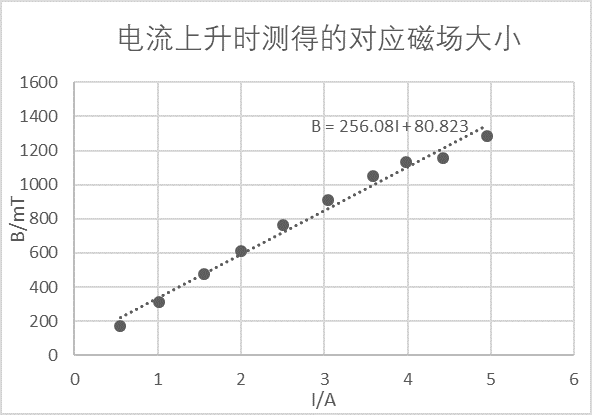
\includegraphics[width=7cm]{上升.png}
}
\subfigure{
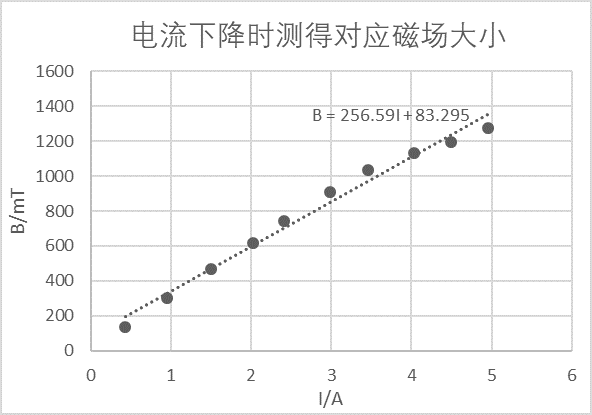
\includegraphics[width=7cm]{下降.png}
}
\end{figure}

\end{document}